\chapter{假设检验} % Introduction chapter suppressed from the table of contents

上章介绍了双样本T检验,是假设检验的一种;下面介绍假设检验,及它帮我们解决什么问题。

%\href{文件:CompareAB1Screenshot_2022-11-06_211947.jpg}{600px}

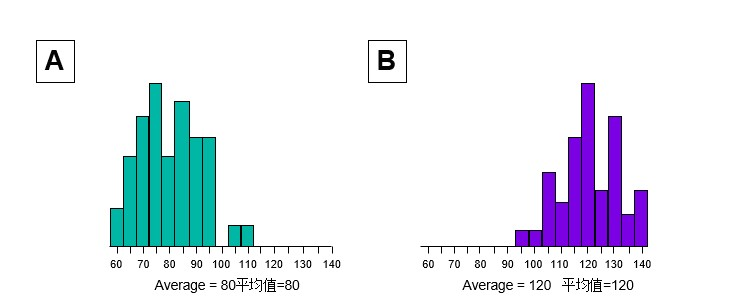
\includegraphics[width=10cm]{CompareAB1Screenshot_2022-11-06_211947.jpg}\\

想比较A B两组 实验结果是否有显著差异。如果像上图
应该看到B很明显比A高。\\
但如果像下图,我就很难看得出来:\\
%\href{文件:CompareAB2Screenshot_2022-11-06_212036.jpg}{600px}

%CompareAB2Screenshot_2022-11-06_212036.jpg

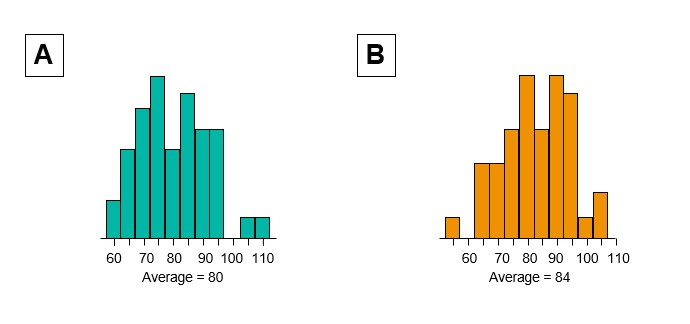
\includegraphics[width=10cm]{CompareAB2Screenshot_2022-11-06_212036.jpg}\\
假设检验利用统计分析方法帮我们区分 - 两组数据是否有显著的差异。

\hypertarget{ux5047ux8bbeux68c0ux9a8cux7684ux6b65ux9aa4}{%
\subsection{假设检验的步骤}\label{ux5047ux8bbeux68c0ux9a8cux7684ux6b65ux9aa4}}

零假设: A 与 B 没有显著差异

备选假设: A 与 B 有显著差异

挑选对应的检验方法后,

可以利用工具计算出的P值来判断:

\begin{description}
\item[]
\begin{description}
\tightlist
\item[]
如果P值大于0.05,就不能拒绝零假设

如果P值小于0.05,就可以拒绝
\end{description}
\end{description}



因A与B都包含非常多样本数据,我们只可以利用A的随机抽样,和B的随机抽样数值,来判断A与B是否有显著差异,这便是双样本T检验。 \\
要深入了解便要与数据,先举个比较简单的假设检验实例:\\

\hypertarget{ux68c0ux9a8cux5355ux4e2aux6b63ux6001ux603bux4f53ux7684ux5747ux503c}{%
\subsection{检验单个正态总体的均值}\label{ux68c0ux9a8cux5355ux4e2aux6b63ux6001ux603bux4f53ux7684ux5747ux503c}}

按历史数据,某厂生产的钢丝折断力是正态分布(平均值=285 , 标准差=4) ,
更换了新的钢材供货商,随机抽取以下10样本,想判断更换供货商后折断力和原先是否有显著提升?

\begin{description}
\item[]
\begin{description}
\tightlist
\item[]
289 , 286 , 285 , 284 , 286 , 285 , 285 , 286 , 298 , 292
\end{description}
\end{description}

从下面样本钢丝折断力柱状图看到10个样本中有七个接近285,有3个是明显大于285,应如何判断是否有显著差异呢?

%\href{文件:1sigmaUnknownHistogram_of_strength.jpg}{500px}\\
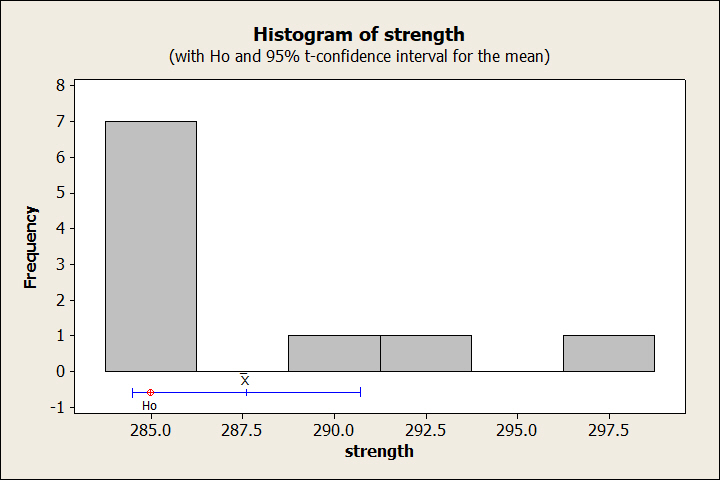
\includegraphics[width=10cm]{1sigmaUnknownHistogram_of_strength.jpg}

按假设检验步骤:

\begin{enumerate}
\tightlist
\item
  零假设*:新钢材的折断力 小于或等于 285
  (\(\mathbf{H}_0: \mu \le 285\))
\item
  备选假设:新钢材的折断力 大于 285 (\(\mathbf{H}_1: \mu > 285\))
\end{enumerate}

\begin{description}
\item[]
\begin{description}
\tightlist
\item[]
(* 通常设零假设为原本情况,没有变化,备选假设为希望的情况,有提升)\\
\end{description}
\end{description}

这例子,可以使用正态分布相关方程式,估计概率, 如概率低于 5\%
,拒绝零假设 ,(折断力 \(> 285\)) (详见附件)\\
如果不想研究相关方程式,可利用概率分布图``看''到:\\
%\href{文件:M4SingleMean1Screenshot_2022-09-11_201026.jpg}{600px}

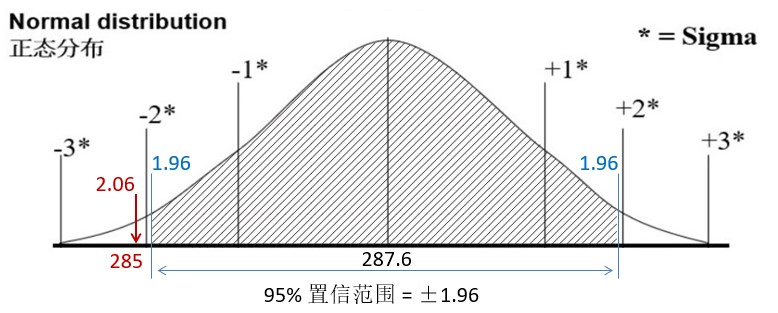
\includegraphics[width=10cm]{M4SingleMean1Screenshot_2022-09-11_201026.jpg}

利用正态概率分布图,抽样的平均值是287.6\\
历史的平均值是285,之间 的差异超出了95\%置信区间,
所以我们拒绝零假设,样本与285 有显著差异(提升)。

也可以利用工具,计算单样本Z检验(one-sample Z test)
的P值,因P值=0.04,少于0.05, 判断拒绝零假设,新供货商的钢丝折断力比原本
285 高。

\framebox{%
\begin{minipage}[t]{0.97\columnwidth}\raggedright
要了解P值是什么?为什么低于0.05可以拒绝? 首先要理解的会发生两类错误

检验可能犯错误,所谓犯错误就是检验的结论与实际情况不符,有两种情况:

\begin{enumerate}
\tightlist
\item
  实际情况是\(\mathbf{H}_0\)成立,而检验的结果表明\(\mathbf{H}_0\)不成立,即拒绝了\(\mathbf{H}_0\),这时称该检验犯了第一类错误(Type
  I error)或``弃真''错误
\item
  实际情况是\(\mathbf{H}_0\)不成立,\(\mathbf{H}_1\)成立,而检验的结果表明\(\mathbf{H}_0\)成立,即接受了\(\mathbf{H}_0\),这时称该检验犯了第二类错误(Type
  II error),或称``取伪''错误
\end{enumerate}

%\href{文件:TypeOneTwoErrorScreenshot_2022-07-23_151744.jpg}{thumb\textbar{}none\textbar{}500px\textbar{}图19}

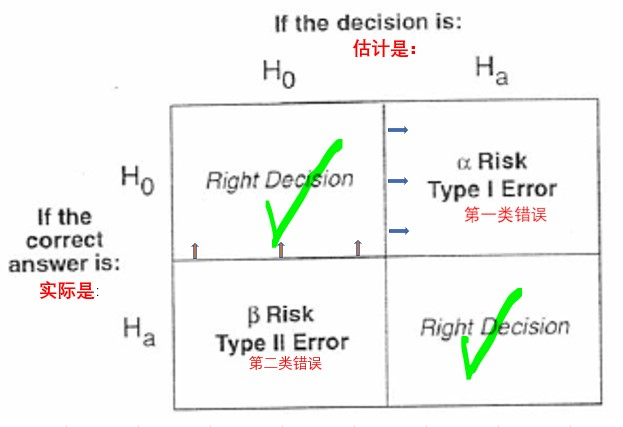
\includegraphics[width=10cm]{TypeOneTwoErrorScreenshot_2022-07-23_151744.jpg}

%这两类错误α与β之间是有关系:\\
%如果α风险(概率从本来0.05 降低)下降, 便会引起
%β风险提高,所以不能同时降低α与β。α不能无限降低,一般选α=0.05 。

这两类错误\(\alpha\) 与\(\beta\) 之间是有关系:\\
如果\(\alpha\) 风险(概率从本来0.05 降低)下降,
便会引起\(\beta\) 风险提高,所以不能同时降低\(\alpha\) 与\(\beta\) 。\(\alpha\) 不能无限降低,一般选\(\alpha\) =0.05 。

%\url{文件:2类错误.jpg}

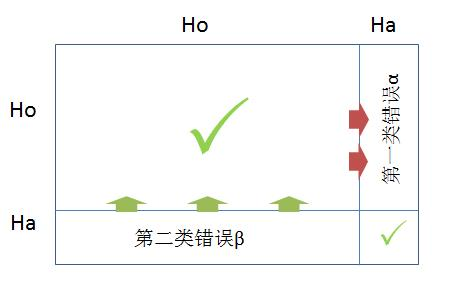
\includegraphics[width=10cm]{2类错误.jpg}

我们可以简单理解P值为发生第一类错误的概率,如果低于5\%我们就有信心拒绝零假设。\strut
\end{minipage}}

假设检验用于比较两组数据有没有显著差异的例子;

\hypertarget{ux6bd4ux8f83ux4e24ux4e2aux6b63ux6001ux603bux4f53ux7684ux5747ux503c}{%
\subsection{比较两个正态总体的均值}\label{ux6bd4ux8f83ux4e24ux4e2aux6b63ux6001ux603bux4f53ux7684ux5747ux503c}}

一名研究人员假设,大学为男生提供的运动项目的平均数量大于大学为女生提供的运动项目的平均数量。对大学为男生和女生提供的体育项目的随机抽样显示,设定临界概率为5\%
(Alpha \(\alpha\)=0.05),是否有足够的证据支持这种说法? (假设方差都一样,
\(\sigma\) = 3.3)。

%Screenshotfrom2022-12-2822-35-57.png

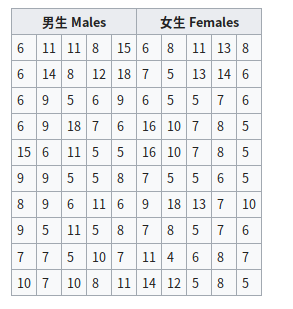
\includegraphics[width=10cm]{Screenshotfrom2022-12-2822-35-57.png}


\begin{enumerate}
\tightlist
\item
  零假设:男女运动项目平均数量没有区别
  (\(\mathbf{H}_0: {\mu}_1 \le  {\mu}_2\))
\item
  备选假设:男生运动项目平均数量比女生多
  (\(\mathbf{H}_1: {\mu}_1 > {\mu}_2\))
\end{enumerate}

男生的均值是 8.6 ; 女生是 7.9 ; 相差是 0.7\\
假定使用90\%置信区间:\\
正态分布 \(\pm 1.65{\sigma}\) (标准差)内的面积是总面积的90\%,从下图看到
1.06 落在90\%置信区间之内,所以不能拒绝零假设。

%\href{文件:M4twoPopulationScreenshot_2022-09-11_201946.jpg}{600px}

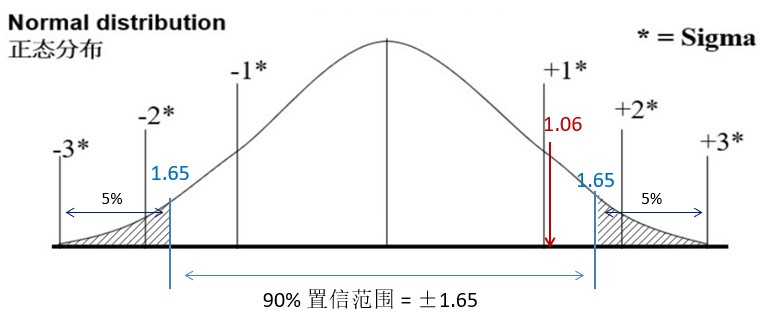
\includegraphics[width=10cm]{M4twoPopulationScreenshot_2022-09-11_201946.jpg}

(有关计算 1.06 的方程式,详见附件)\\
使用工具跑出来的P值是 0.146 , 大于 0.05 ,所以不能拒绝零假设

以上两个例子都是假定:分布的方差已知

但很多时,我们不一定知道分布的方差或标准差是多少?
我们便需要从样本数估计分布的方差(或标准差)。
下面是一个结对T检验(Paired T test)例子

\hypertarget{ux68c0ux9a8cux5355ux4e2aux6b63ux6001ux603bux4f53ux7684ux5747ux503cux65b9ux5deeux672aux77e5}{%
\subsection{检验单个正态总体的均值,方差未知}\label{ux68c0ux9a8cux5355ux4e2aux6b63ux6001ux603bux4f53ux7684ux5747ux503cux65b9ux5deeux672aux77e5}}

营养师正在观察如果每天饮食都添加某类矿物质,是否会改变人的胆固醇水平。对随机选取6位对象在实验之前进行了水平测试。然后对他们进行为期6周的测试,在它们大食物里添加矿物质补充,实验之后再测试,结果显示在下表
(胆固醇水平以每分升毫克为单位)。能否得出结论,在α=
0.1时,胆固醇水平是否发生了变化。

%Screenshotfrom2022-12-2822-37-19.png

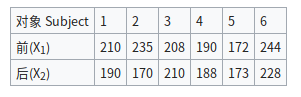
\includegraphics[width=10cm]{Screenshotfrom2022-12-2822-37-19.png}

\begin{enumerate}
\tightlist
\item
  零假设:没有变化 (\(\mathbf{H}_0: \mu _D = 0\))
\item
  备选假设:有显著变化 (\(\mathbf{H}_1: \mu _D \neq 0\))
\end{enumerate}

注意:与上面大学男女生的各50个数据成一组, 两组50个数之间没有对应关系

这例子不一样, 因前后是一一对应, 我们需要用结对T检验 (Paired T test)。
因标准差不是已知,是从样本估算,所以要用 T检验,非 Z检验。

可以使用相关方程式,计算出 T值 =1.61 ,

%\href{文件:CholesterolEg2022-07-23_195121.jpg}{thumb\textbar{}none\textbar{}500px\textbar{}图20}

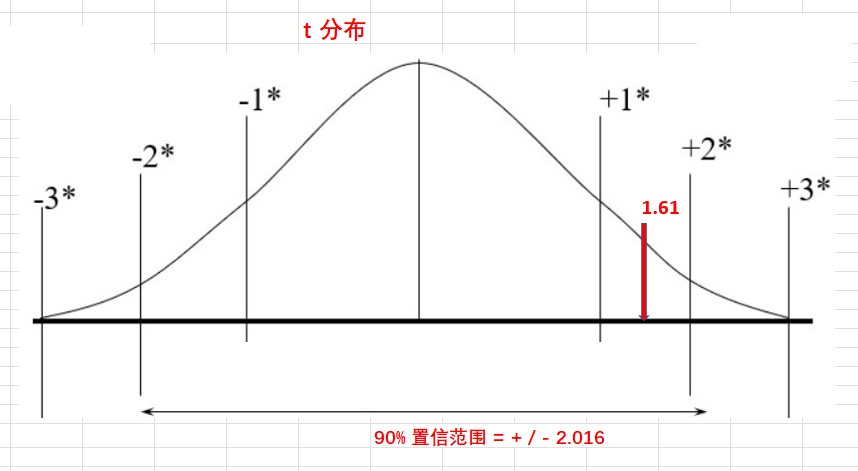
\includegraphics[width=10cm]{CholesterolEg2022-07-23_195121.jpg}

从上图看到 1.61 落在90\%置信区间(2.016)之内,所以不能拒绝零假设。

也可以利用工具,计算双样本T检验(Paired T test)
的P值,因P值=0.165,大于0.05, 判断不能拒绝零假设

如果想比较比较超过两组数据便要用方差分析(ANOVA)

\hypertarget{ux65b9ux5deeux5206ux67901-anova-test}{%
\subsection{方差分析(ANOVA
test)}\label{ux65b9ux5deeux5206ux67901-anova-test}}

\hypertarget{ux65b9ux5deeux5206ux67902-anova-test}{%
\subsubsection{例子一}\label{ux65b9ux5deeux5206ux67902-anova-test}}

比较三种车型(小轿车,舒适型 , 豪华车)的省油系数有没有显著差异?\\
%\href{文件:5anovaDataScreenshot_2022-07-24_105955.jpg}{文件:5anovaDataScreenshot
%2022-07-24 105955.jpg}\\
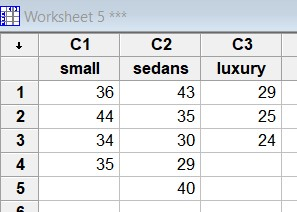
\includegraphics[width=10cm]{5anovaDataScreenshot_2022-07-24_105955.jpg}\\
用统计工具跑单因子方差分析
得出P值是0.0385,低于0.05,所以我们便可以拒绝零假设 

%\href{文件:5anovaResultScreenshot_2022-07-24_104352.jpg}{400px}\\

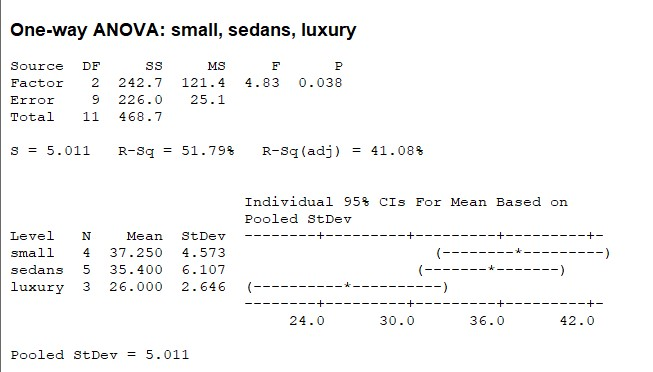
\includegraphics[width=10cm]{5anovaResultScreenshot_2022-07-24_104352.jpg}\\
从下面工具的简单画图的也看到豪华型的系数范围比其他两种有显著差异:

%\href{文件:5anovaBoxplot_of_small,_sedans,_luxury.jpg}{500px}\\

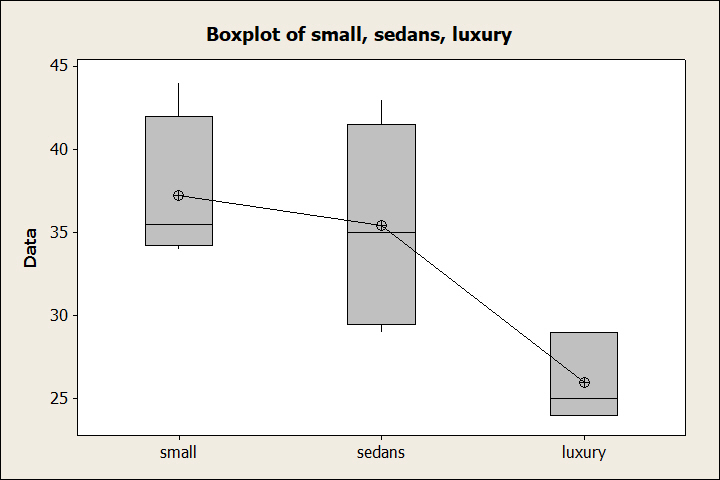
\includegraphics[width=10cm]{5anovaBoxplot_of_small_sedans_luxury.jpg}\\
方差分析只能识别有没有显著差异,但若要要明确哪些地方有差异,便要用
Tukey-Kramer 做多组之间比较

%\hypertarget{ux65b9ux5deeux5206ux67902-anova-test}{%
%\subsubsection{例子二}\label{ux65b9ux5deeux5206ux67902-anova-test}}

\hypertarget{ux65b9ux5deeux5206ux67902-anova-test}{%
\subsubsection{方差分析2 (ANOVA
test)}\label{ux65b9ux5deeux5206ux67902-anova-test}}

某降落伞工厂想比较4家布料供货商的布料拉力
(因拉力不足会影响使用者的性命安全)\\
下面是它们随机抽样的结果:

%Screenshotfrom2022-12-2822-39-42.png

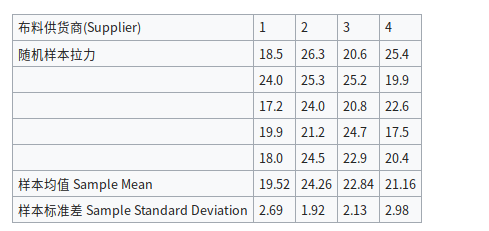
\includegraphics[width=10cm]{Screenshotfrom2022-12-2822-39-42.png}

用工具跑方差分析P值是0.042,少于0.05, 判断拒绝零假设

\begin{itemize}
\tightlist
\item
  Minitab 出来方差分析结果表,与上面的总结表能一一对应;
\end{itemize}

%\href{文件:AnovaParachutes807Screenshot_2022-08-07_124737.jpg}{400px}

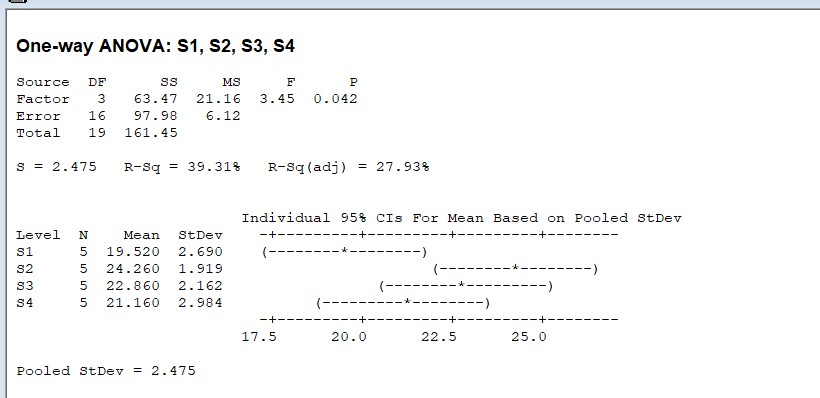
\includegraphics[width=10cm]{AnovaParachutes807Screenshot_2022-08-07_124737.jpg}

%\href{文件:AnovaBoxplots807.jpg}{400px}

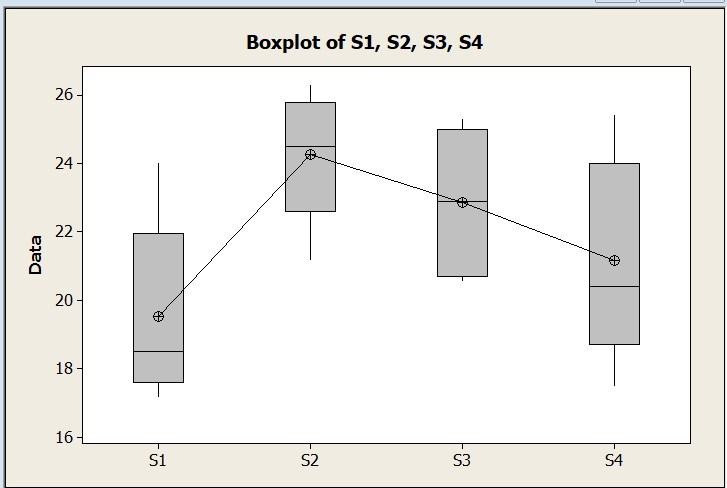
\includegraphics[width=10cm]{AnovaBoxplots807.jpg}

%\href{文件:Anova3inOneScreenshot_2022-08-07_125131.jpg}{400px}

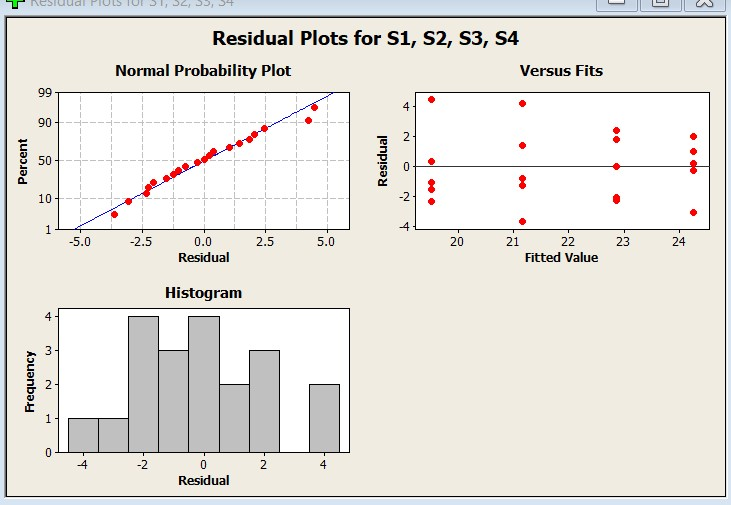
\includegraphics[width=10cm]{Anova3inOneScreenshot_2022-08-07_125131.jpg}

\begin{itemize}
\tightlist
\item
  从4组的分布,你可能看出第一组与第二组的差异很明显,其他差不多。但当差异没有这么明显,便需要用统计分析判断。
\end{itemize}

\hypertarget{tukey-kramer-ux591aux7ec4ux6bd4ux8f83}{%
\subsubsection{Tukey-Kramer
多组比较}\label{tukey-kramer-ux591aux7ec4ux6bd4ux8f83}}

\textbf{实例}(比较4供货商布料的拉力):\\
\#\(|\overline{X_1} - \overline{X_2}\) = \textbar{}19.52 --
24.26\textbar{} = 4.74

\begin{enumerate}
\tightlist
\item
  \(|\overline{X_1} - \overline{X_3}\) = \textbar{}19.52 --
  22.84\textbar{} = 3.32
\item
  \(|\overline{X_1} - \overline{X_4}\) = \textbar{}19.52 --
  21.16\textbar{} = 1.64
\item
  \(|\overline{X_2} - \overline{X_3}\) = \textbar{}24.26 --
  22.84\textbar{} = 1.42
\item
  \(|\overline{X_2} - \overline{X_4}\) = \textbar{}24.26 --
  21.16\textbar{} = 3.10
\item
  \(|\overline{X_3} - \overline{X_4}\) = \textbar{}22.84 --
  21.16\textbar{} = 1.68
\end{enumerate}

用Tukey-Kramer 相关方程式(详见附件),得出临界范围为 4.47,所以判断唯一供货商1与2的布料拉力是有显著差异。 

%\hypertarget{ux5206ux7ec4ux5206ux7c7bux6570ux636e}{%
%\section{分组(分类)数据}\label{ux5206ux7ec4ux5206ux7c7bux6570ux636e}}

\hypertarget{ux65b9ux5deeux5206ux67901-anova-test}{%
\subsection{分组(分类)数据}\label{ux65b9ux5deeux5206ux67901-anova-test}}

上面都是用于连续数据的例子

假设检验也可以用于分组(分类)数据

\hypertarget{ux5361ux65b9ux68c0ux9a8cchi-square-test}{%
\subsubsection{卡方检验(Chi Square
test)}\label{ux5361ux65b9ux68c0ux9a8cchi-square-test}}

想研究三家医院针在 三类病人感染的主因:(外科手术 Surgical Site , 肺炎
Pneumonia, 血液 Bloodstream) 最终导致病人死亡

是否有显著差异?

%\href{文件:4chiSquareDataScreenshot_2022-07-24_110053.jpg}{文件:4chiSquareDataScreenshot
%2022-07-24 110053.jpg}\\

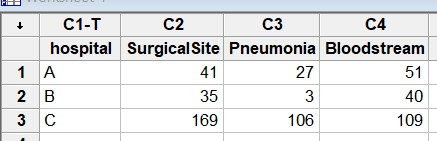
\includegraphics[width=6cm]{4chiSquareDataScreenshot_2022-07-24_110053.jpg}

\begin{enumerate}
\tightlist
\item
  零假设:那家医院与感染主因没有关系
\item
  备选假设:有显著关系
\end{enumerate}

卡方检验得出P值等于零,所以可以拒绝零假设,医院与感染主因有关系

%\href{文件:6chiSquareTstResultScreenshot_2022-07-24_103606.jpg}{500px}\\

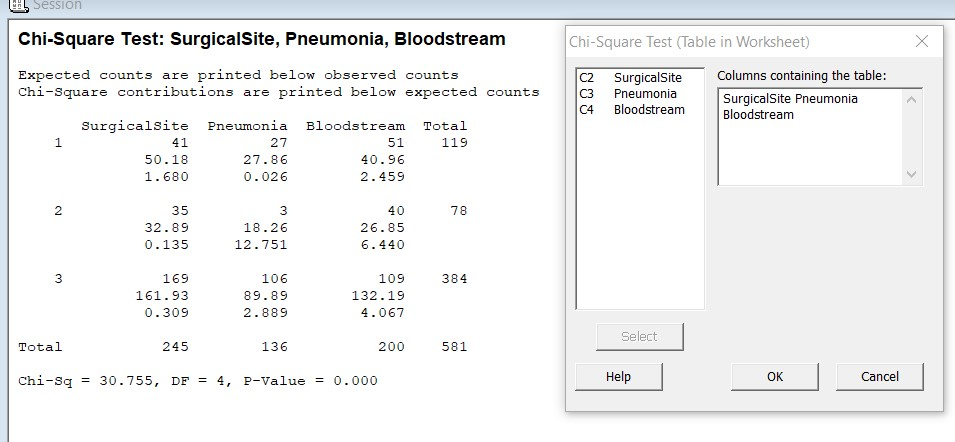
\includegraphics[width=6cm]{6chiSquareTstResultScreenshot_2022-07-24_103606.jpg}

1:零假设:医院(Hospitals) 与 感染种类(Infections) 之间没有相关

2:为了计算卡方值(Chi-square),首先使用以下公式计算每个列联表的预计值E(Expected
Value),

\(E = \frac{(row \ sum) * (column \ sum)} {grand \ total}\)

再用下面公式从预计值与实际值O(Observed value),计算卡方值 :

\(\chi ^2 = \sum \frac{(O - E)^2} {E}\)

3:计算得出卡方值 = 30.696 (注) ,比 关键值 9.5 高

\begin{description}
\tightlist
\item[]
(对应 DF=4 (=(3-1)*(3-1))
,\(\alpha = 0.05\),从\(\chi ^2\)统计表得出9.5),\\
\end{description}

所以拒绝零假设,医院(Hospitals) 与 感染种类(Infections) 之间相关。\\

(注:对应 Minitab 工具自动算出的 30.755)\\

\hypertarget{ux9644ux4ef6}{%
\section{附件}\label{ux9644ux4ef6}}

\hypertarget{ux68c0ux9a8cux5355ux4e2aux6b63ux6001ux6574ux4f53ux5747ux503cux76f8ux5173ux65b9ux7a0bux5f0f}{%
\subsection{检验单个正态整体均值相关方程式}\label{ux68c0ux9a8cux5355ux4e2aux6b63ux6001ux6574ux4f53ux5747ux503cux76f8ux5173ux65b9ux7a0bux5f0f}}

平均值分布的方 = 样本方差 / n ,并可以用以下方程式估算(如果样本数n
越大,样本均值的方差就越少):

\(Z_n = \cfrac{ \sqrt{n}(\overline{X_n} - \mu) }{\sigma}\)\\

\(\overline{X} = 287.6\)

\(\cfrac{ \sqrt{n}(\overline{X} - \mu_0) }{\sigma} = \cfrac{ \sqrt{10}( 287.6 - 285 ) }{4} = 2.06\)\\

\hypertarget{ux6bd4ux8f83ux4e24ux4e2aux6b63ux6001ux603bux4f53ux7684ux5747ux503c-1}{%
\subsection{比较两个正态总体的均值}\label{ux6bd4ux8f83ux4e24ux4e2aux6b63ux6001ux603bux4f53ux7684ux5747ux503c-1}}

\begin{description}
\tightlist
\item[]
男生:
\end{description}

\(\overline{X_1} = 8.6\) ; \(\overline{\sigma_1} = 3.3\)\\
女生: \(\overline{X_2} = 7.9\) ; \(\overline{\sigma_2} = 3.3\)\\

\[\cfrac{ (\overline{X_1} - \overline{X_2}) - ({\mu}_1  - {\mu}_2)}{\sqrt{\cfrac{\sigma_1^2}{n_1} + \cfrac{\sigma_2^2}{n_2}}} = \cfrac{ (8.6 - 7.9) - 0 }{\sqrt{\cfrac{(3.3)^2}{50} + \cfrac{(3.3)^2}{50}}} = 1.06\]

\hypertarget{ux68c0ux9a8cux5355ux4e2aux6b63ux6001ux603bux4f53ux7684ux5747ux503cux65b9ux5deeux672aux77e5-1}{%
\subsection{检验单个正态总体的均值,方差未知}\label{ux68c0ux9a8cux5355ux4e2aux6b63ux6001ux603bux4f53ux7684ux5747ux503cux65b9ux5deeux672aux77e5-1}}

\(\overline{D} = \sum D / n = 100/6 = 16.7\)\\
(\(D = X_1 - X_2\) )\\
\(\mathbf{H}_0\)的拒绝域为:\\
\(\cfrac{ \sqrt{n}(\overline{D} - \mu _0) }{S_D}  > t_\alpha(n-1)\)\\

\begin{itemize}
\tightlist
\item
  查student-t 分布表,\(t_{0.05} (5) = 2.016\)
\item
  从样本估计方差\\
\end{itemize}

\(s_D^2 = \cfrac{\sum {(D_i - \overline{D})}^2  }{(n - 1)}= \cfrac{\sum D_i^2 - n \times \overline{D}^2  }{(n - 1)} = \cfrac{4890 - 6 \times (16.7)^2  }{(6 - 1)} = 645\)\\
\(s_D = 25.4\)\\

\begin{itemize}
\tightlist
\item
  计算得:
\end{itemize}

\(t = \cfrac{ \sqrt{n}(\overline{D} - \mu _0) }{S_D} = \cfrac{ \sqrt{6}(16.7 - 0) }{25.4}\)\\
= 1.61\\




\hypertarget{tukey-kramer-ux76f8ux5173ux65b9ux7a0bux5f0f}{%
\subsection{Tukey-Kramer
相关方程式}\label{tukey-kramer-ux76f8ux5173ux65b9ux7a0bux5f0f}}

\begin{itemize}
\tightlist
\item
  计算显著差异的临界值:
\end{itemize}

\begin{description}
\item[]
\begin{description}
\tightlist
\item[]
Critical range=
\(Q_u \sqrt{{MSW \over 2} ({1\over n_j} +{1\over n_j '})}\)

对应布料拉力例子:\\
\(\alpha\) = 0.05, c = 4 , n - c= 20-4 = 16\\
从统计表 得出对应 \(Q_u\) = 4.05 ;\\ MSW =6.1 (如何计算MSW,
详见下面"如何计算 MSW")

代入上面方程式:

\begin{description}
\item[]
\begin{description}
\tightlist
\item[]
Critical range=
\(4.05 \sqrt{({6.1 \over 2}) ({1\over 5} + {1\over 5 })}\)
\end{description}
\end{description}

\begin{description}
\item[]
\begin{description}
\tightlist
\item[]
= 4.47
\end{description}
\end{description}

\hypertarget{ux5982ux4f55ux8ba1ux7b97-mswux53c2ux8003anovaux65b9ux7a0bux5f0f}{%
\subsubsection{如何计算
MSW,参考ANOVA方程式}\label{ux5982ux4f55ux8ba1ux7b97-mswux53c2ux8003anovaux65b9ux7a0bux5f0f}}

\begin{itemize}
\tightlist
\item
  总离差平方和 Total Variation = Sum of Squares for Total (SST):
\end{itemize}

\begin{itemize}
\tightlist
\item
  SST 由 组内离差平方和(SSW), 和 组间离差平方和(SSA), 双加出来:
\end{itemize}

\begin{itemize}
\tightlist
\item
  组间离差平方和 (SSA)
\end{itemize}

\begin{itemize}
\tightlist
\item
  组内离差平方和 (SSW)
\end{itemize}

\begin{itemize}
\tightlist
\item
  如果组间离差远远大于组内离差,表示组间差异大,应拒绝零假设;反之,如差异不大,便难以拒绝零假设,没有显著差异。
\end{itemize}

\begin{itemize}
\tightlist
\item
  单因素方差分析 计算 F = MSA / MSW , 如果F值大于临界值,拒绝零假设
\end{itemize}

能直接算出下面总结报告:\\

%Screenshotfrom2023-02-1401-07-07.png

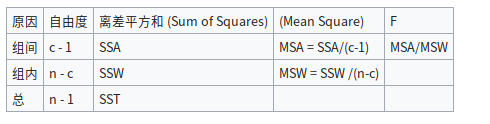
\includegraphics[width=6cm]{Screenshotfrom2023-02-1401-07-07.png}

\textbf{相关方程式}\\
* 总离差平方和\\
SST =
\(\sum_{j=1}^c \sum_{i=1}^{n_j} (X_{ij} - \overline{\overline{X}})^2\)
\end{description}
\end{description}

\begin{description}
\item[]
\begin{description}
\tightlist
\item[]
注: 总体平均数
\(\overline{\overline{X}} = {\sum_{j=1}^c \sum_{i=1}^{n_j} X_{ij} \over n }\)
\end{description}
\end{description}

\begin{itemize}
\tightlist
\item
  组间离差平方和\\
\end{itemize}

\texttt{SSA~=~}\(\sum_{j=1}^c n_j(\overline{X_j} - \overline{\overline{X}})^2\)

\begin{description}
\item[]
\begin{description}
\tightlist
\item[]
注: 组j的平均值 \(\overline{X_j}\)
\end{description}
\end{description}

\begin{itemize}
\tightlist
\item
  组内离差平方和\\
\end{itemize}

\texttt{SSW~=~}\(\sum_{j=1}^c \sum_{i=1}^{n_j} (X_{ij} - \overline{X_j})^2\)

\begin{description}
\item[]
\begin{description}
\tightlist
\item[]
注: 组j的平均值 \(\overline{X_j}\)
\end{description}
\end{description}

\begin{itemize}
\tightlist
\item
  单因素方差分析 均方和
\end{itemize}

\texttt{MSA~=~}\({SSA \over c -1}\)

\texttt{MSW~=~~}\({SSW \over n -c}\)

\texttt{MST~=~}\({SST \over n -1}\)

\textbf{实例}(比较4供货商布料的拉力):

\begin{itemize}
\tightlist
\item
  组间自由度 = c - 1 = 4 - 1 =3
\item
  组内自由度 = n - c = 20 - 4 =16
\item
  总自由度 = n - 1 = 20-1 = 19
\end{itemize}

总体平均数
\(\overline{\overline{X}} = {\sum_{j=1}^c \sum_{i=1}^{n_j} X_{ij} \over n} = {438.9 \over 20}= 21.945\)

SSA = \(\sum_{j=1}^c n_j(\overline{X_j} - \overline{\overline{X}})^2\)

\[= (5)(19.52 - 21.945)^2 + (5)(24.26 - 21.945)^2 + (5)(22.84 - 21.945)^2 + (50(21.16 - 21.945)^2\]

\[= 63.285\]

SSW = \(\sum_{j=1}^c \sum_{i=1}^{n_j} (X_{ij} - \overline{X_j})^2\)

\[=(18.5 - 19.52)^2 + . . + (18.0 - 19.52)^2 + (26.3 - 24.26)^2 + . . + (24.5 - 24.26)^2\]

\[+(25.4 - 21.16)^2 + . . + (20.4 - 21.16)^2\]

\[= 97.5\]

SST =
\(\sum_{j=1}^c \sum_{i=1}^{n_j} (X_{ij} - \overline{\overline{X}})^2\)

\[= (18.5 - 21.945)^2 + (24 - 21.945)^2 + ..+ (20.4 - 21.945)^2\]

\[= 160.7895\]

MSA = \({SSA \over c-1}\) = \({63.285 \over 4-1}\) = 21.1\\
MSW = \({SSW \over n -c} = {97.5 \over 16}= 6.1\)\\
F = MSA / MSW = 21.1 / 6.1 = 3.46\\
能对应文中 Minitab 出来的结果:\\
MSA = 21.16, MSW = 6.12, F = 3.45\\

